% !TeX root = ../main.tex
\section{Technische Grundlagen}
\label{cap:grundlagen}

Die nachfolgenden technischen Grundlagen dienen dazu, die für diese Arbeit relevanten Zusammenhänge zu erläutern.

\subsection{Erstes Grundlagenthema}
\label{cap:grundlage1}

Fließtext mit Quellenangabe~\cite{bachelorarbeit} und einer Fußnote\footnote{Fußnoten erscheinen wie in der BA immer am Seitenende.}.

Formeln werden nummeriert und mit Label versehen, siehe Gleichung~\eqref{eq:scherfestigkeit}:

\begin{equation}
	\label{eq:scherfestigkeit}
	\tau = \frac{F_{\text{max}}}{A_{\text{Bond}}}
\end{equation}

Einheiten immer mit \texttt{siunitx} setzen, z.\,B. \SI{1,2}{\milli\meter}, \SI{50}{\micro\meter\per\second} oder \SIrange{425}{450}{\celsius}.

Abbildung~\ref{fig:beispiel} zeigt ein Beispielbild.

\begin{figure}[H]
	\centering
	% Eigene Bilder in abbildungen/<Unterordner>/ ablegen,
	% möglichst ohne Leerzeichen und Umlaute im Dateinamen.
	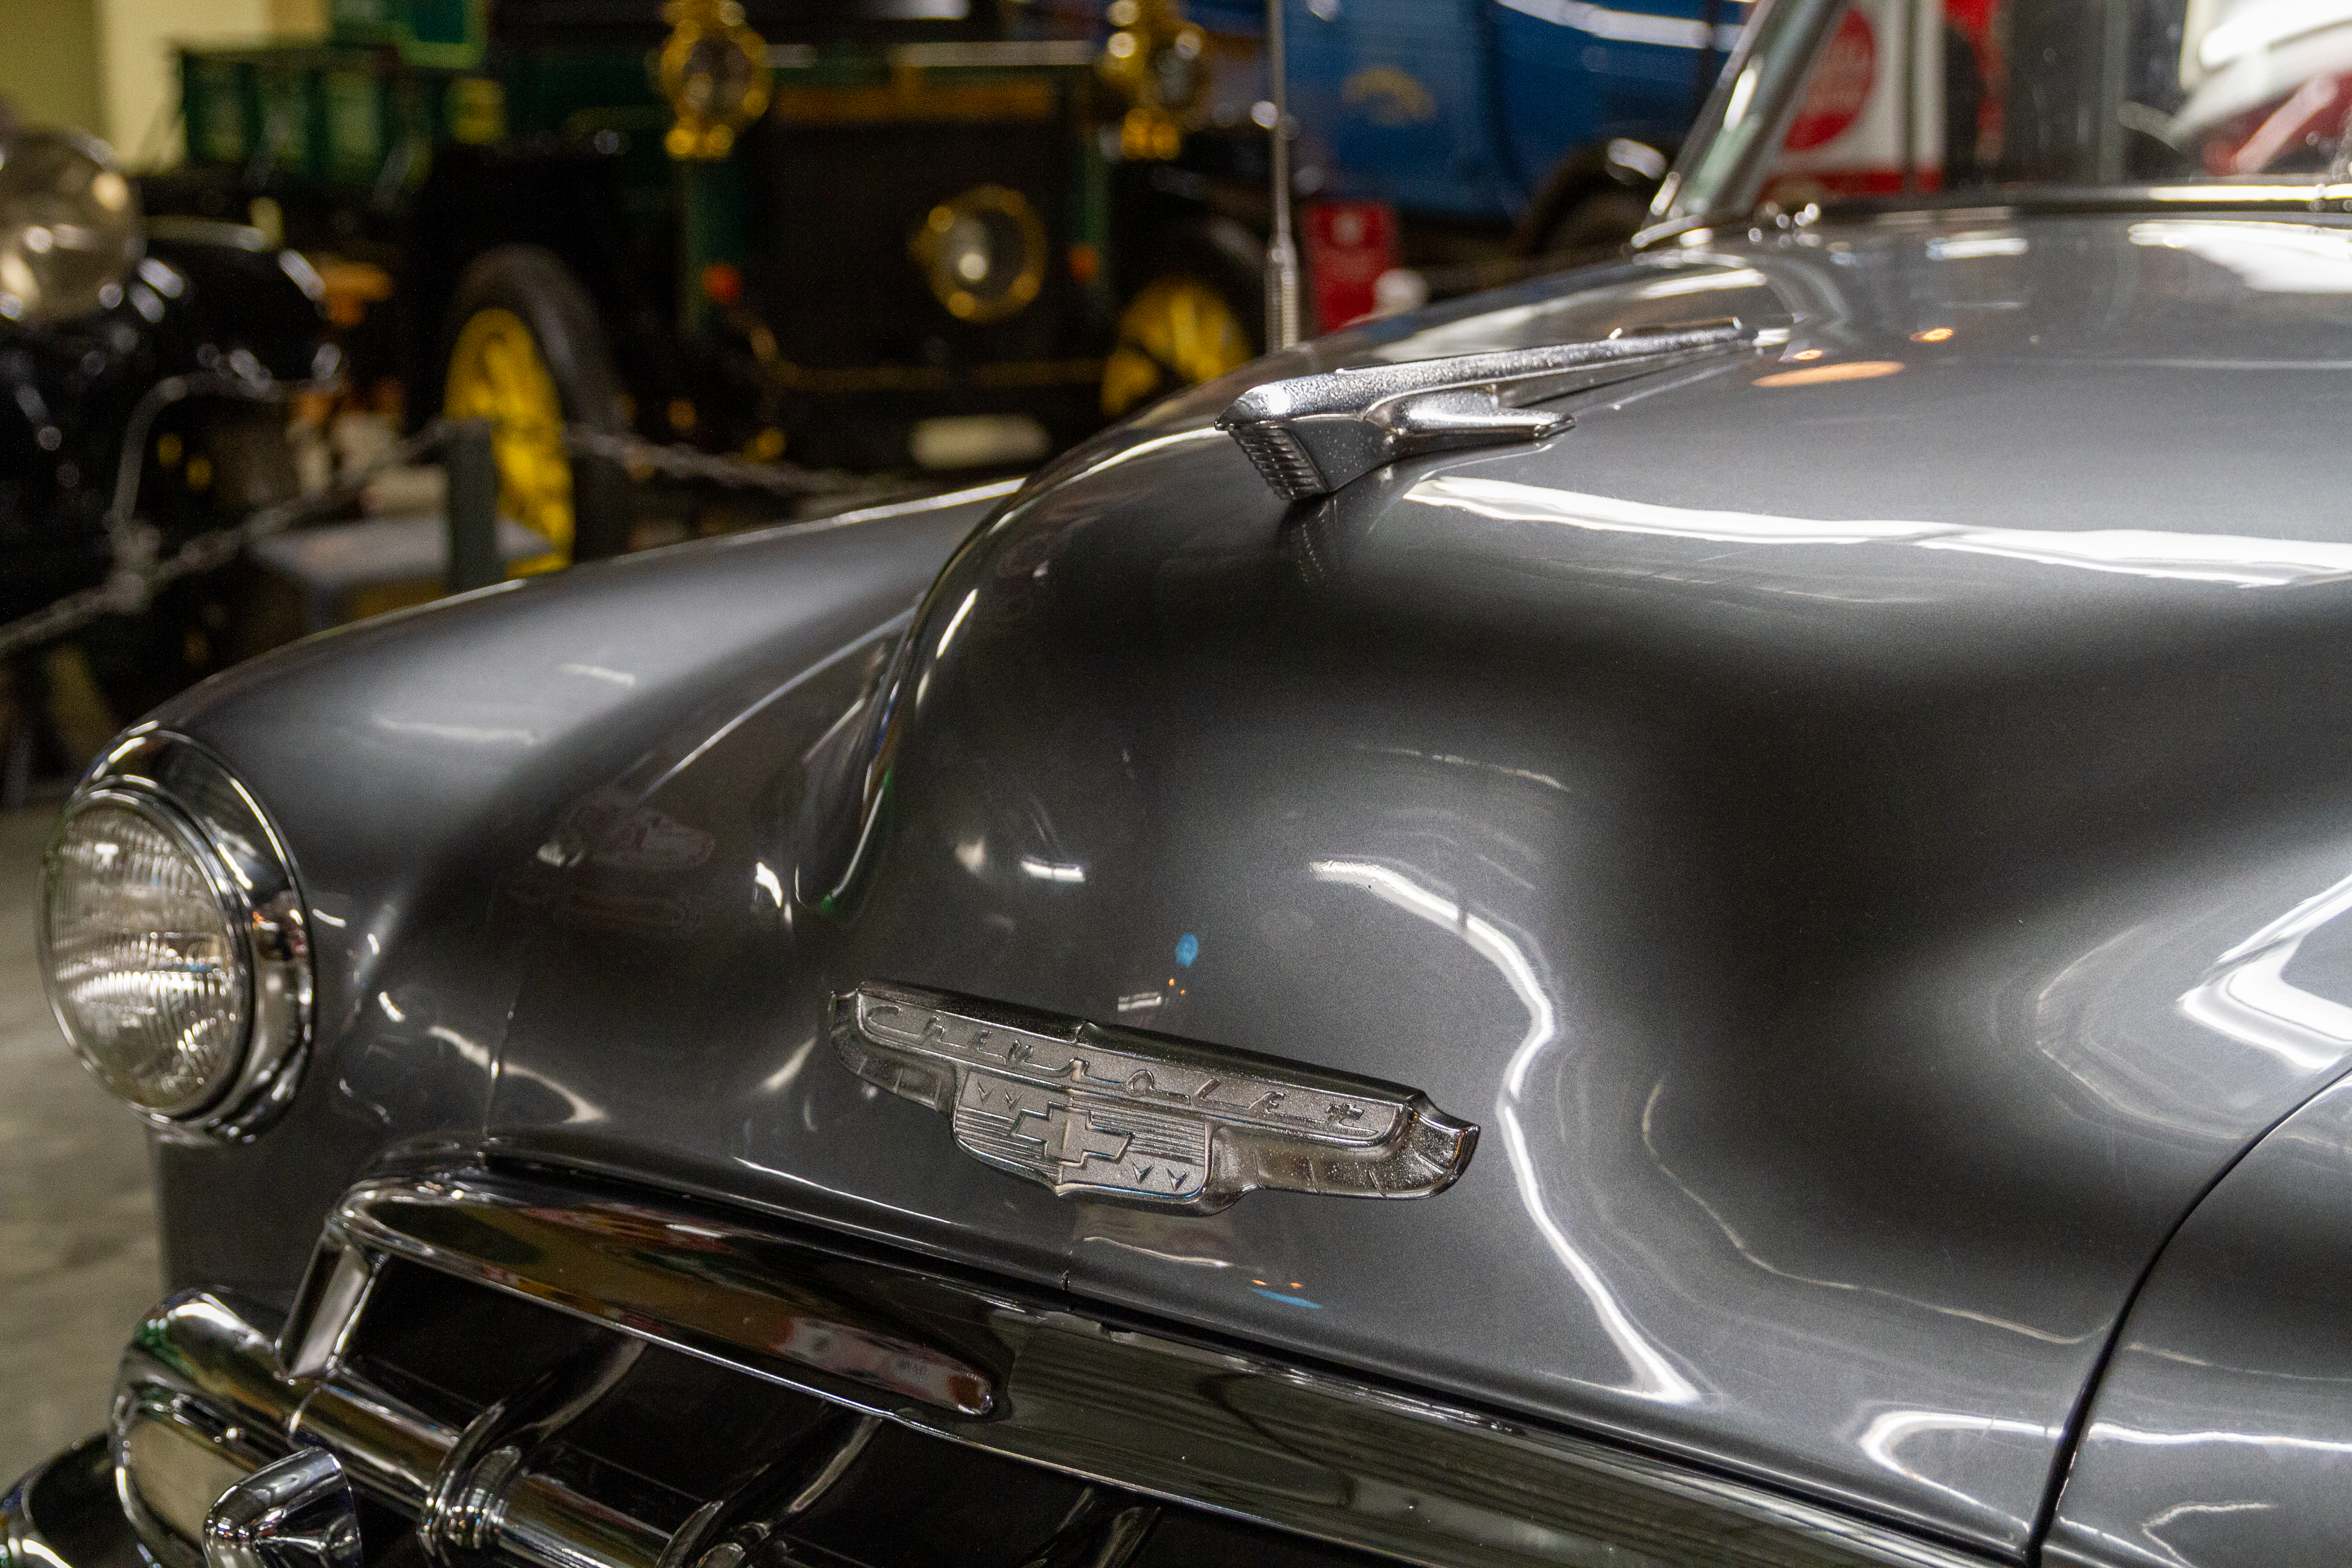
\includegraphics[width=0.6\textwidth]{example-image-a}
	\caption[Kurzer Titel fürs Abbildungsverzeichnis]{Ausführliche Bildunterschrift, die im Text erscheint}
	\label{fig:beispiel}
\end{figure}

\subsection{Zweites Grundlagenthema}
\label{cap:grundlage2}

\subsubsection{Unterpunkt}

Text.

\paragraph{Absatzüberschrift:}
Text.
